\documentclass[11pt,oneside]{article}

\pdfminorversion=7
\usepackage{QuizStyle}
\usepackage{tikz}

\hypersetup{
    pdftitle={20261015 Quiz for MATH102 Calculus II},
    pdfauthor={Jungwoo Kim},
    pdfsubject={Quiz for MATH102 Calculus II},
    pdfcreator={LaTeX}
}

\begin{document}

\quiztitle{20261015 Quiz}

\begin{problem}{3.15}
Find an equation for the plane tangent to the graph of $f(x,y)=x+y^2$,
\begin{problemsubparts}
    \item at $(x,y)=(0,0)$,
    \item at $(x,y)=(1,2)$.
\end{problemsubparts}
\end{problem}

\begin{solution}
Since $f_x(x,y)=1$ and $f_y(x,y)=2y$, the tangent plane at $(a,b,f(a,b))$ is
\[
    z=f(a,b)+f_x(a,b)(x-a)+f_y(a,b)(y-b).
\]
\begin{problemsubparts}
    \item At $(0,0)$, we have $f(0,0)=0$, $f_x(0,0)=1$, and $f_y(0,0)=0$. Hence
    \[
        \boxed{z=x}.
    \]

    \item At $(1,2)$, we have $f(1,2)=5$, $f_x(1,2)=1$, and $f_y(1,2)=4$. Thus
    \[
        \boxed{z=5+(x-1)+4(y-2)}.
    \]
\end{problemsubparts}
\end{solution}

\begin{problem}{3.16}
Let
\[
    f(x,y)=\sqrt{1-x^2-y^2}.
\]
\begin{problemsubparts}
    \item Sketch the graph of $f$.
    \item Find an equation of the plane tangent to the graph of $f$ at $(x,y)=(\sqrt{0.4},\sqrt{0.5})$.
\end{problemsubparts}
\end{problem}

\begin{solution}
\begin{problemsubparts}
    \item Since $z=f(x,y)\geq0$ and
    \[
        x^2+y^2+z^2=1,
    \]
    the graph is the upper hemisphere of the unit sphere, including its boundary circle $x^2+y^2=1$ in the plane $z=0$.

    \begin{center}
    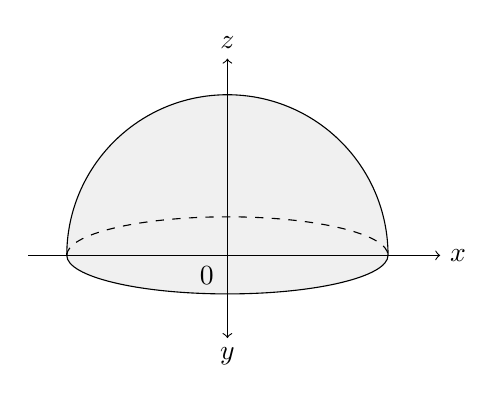
\begin{tikzpicture}[scale=1.02]
        \fill[black!6] (-2,0) arc[start angle=180,end angle=0,radius=2]
            arc[start angle=0,end angle=-180,x radius=2,y radius=0.48] -- cycle;
        \draw[->] (-2.48,0) -- (2.65,0) node[right] {$x$};
        \draw[->] (0,0) -- (0,-1.03) node[below] {$y$};
        \draw[->] (0,0) -- (0,2.45) node[above] {$z$};
        \draw[dashed] (-2,0) arc[start angle=180,end angle=0,x radius=2,y radius=0.48];
        \draw (-2,0) arc[start angle=180,end angle=0,radius=2];
        \draw (-2,0) arc[start angle=180,end angle=360,x radius=2,y radius=0.48];
        \node[below left] at (-0.05,-0.02) {$0$};
    \end{tikzpicture}
    \end{center}

    \item Put $a=\sqrt{0.4}=\sqrt{\frac25}$ and $b=\sqrt{0.5}=\frac1{\sqrt2}$. Then
    \[
        f(a,b)=\sqrt{1-\frac25-\frac12}=\frac1{\sqrt{10}}.
    \]
    In the interior of the unit disk,
    \[
        f_x(x,y)=-\frac{x}{\sqrt{1-x^2-y^2}},
        \qquad
        f_y(x,y)=-\frac{y}{\sqrt{1-x^2-y^2}}.
    \]
    Consequently,
    \[
        f_x(a,b)=-2,
        \qquad
        f_y(a,b)=-\sqrt5.
    \]
    The tangent plane is therefore
    \[
        z=\frac1{\sqrt{10}}-2(x-a)-\sqrt5(y-b),
    \]
    or, equivalently,
    \[
        \boxed{2x+\sqrt5\,y+z=\sqrt{10}}.
    \]
\end{problemsubparts}
\end{solution}

\begin{problem}{3.18}
Find the following derivatives or partial derivatives.
\begin{problemsubparts}
    \item $\dfrac{\dd}{\dd x}\bigl(f(x)^3\bigr)$, where $f\colon\R\to\R$ is differentiable.
    \item $\dfrac{\partial}{\partial x}(y+x^2)^3$.
    \item $\dfrac{\partial}{\partial x}g(y+x^2)$, where $g\colon\R\to\R$ is differentiable.
    \item $\dfrac{\partial}{\partial y}\bigl(f(x,y)^3\bigr)$, where $f\colon\R^2\to\R$ is differentiable.
\end{problemsubparts}
\end{problem}

\begin{solution}
Applying the Chain Rule, with the other variable held fixed for partial derivatives, gives
\begin{problemsubparts}
    \item
    \[
        \boxed{\frac{\dd}{\dd x}\bigl(f(x)^3\bigr)=3f(x)^2f'(x)}.
    \]

    \item
    \[
        \boxed{\frac{\partial}{\partial x}(y+x^2)^3=6x(y+x^2)^2}.
    \]

    \item
    \[
        \boxed{\frac{\partial}{\partial x}g(y+x^2)=2xg'(y+x^2)}.
    \]

    \item
    \[
        \boxed{\frac{\partial}{\partial y}\bigl(f(x,y)^3\bigr)=3f(x,y)^2f_y(x,y)}.
    \]
\end{problemsubparts}
\end{solution}

\begin{problem}{3.19}
Find the derivatives $f_{xx}$, $f_{xy}$, and $f_{yy}$ for each function.
\begin{problemsubparts}
    \item $f(x,y)=x^2-y^2$.
    \item $f(x,y)=x^2+y^2$.
    \item $f(x,y)=(x+y)^2$.
    \item $f(x,y)=e^{-x}\cos y$.
    \item $f(x,y)=e^{-ay}\sin(ax)$, where $a$ is a constant.
\end{problemsubparts}
\end{problem}

\begin{solution}
\begin{problemsubparts}
    \item Here $f_x=2x$ and $f_y=-2y$, so
    \[
        \boxed{f_{xx}=2,\qquad f_{xy}=0,\qquad f_{yy}=-2}.
    \]

    \item Here $f_x=2x$ and $f_y=2y$, so
    \[
        \boxed{f_{xx}=2,\qquad f_{xy}=0,\qquad f_{yy}=2}.
    \]

    \item Here $f_x=2(x+y)=f_y$, so
    \[
        \boxed{f_{xx}=2,\qquad f_{xy}=2,\qquad f_{yy}=2}.
    \]

    \item Since
    \[
        f_x=-e^{-x}\cos y,
        \qquad
        f_y=-e^{-x}\sin y,
    \]
    we obtain
    \[
        \boxed{f_{xx}=e^{-x}\cos y,\quad f_{xy}=e^{-x}\sin y,\quad f_{yy}=-e^{-x}\cos y}.
    \]

    \item Since
    \[
        f_x=ae^{-ay}\cos(ax),
        \qquad
        f_y=-ae^{-ay}\sin(ax),
    \]
    we obtain
    \[
        \boxed{\begin{aligned}
            f_{xx}&=-a^2e^{-ay}\sin(ax),\\
            f_{xy}&=-a^2e^{-ay}\cos(ax),\\
            f_{yy}&=a^2e^{-ay}\sin(ax).
        \end{aligned}}
    \]
\end{problemsubparts}
\end{solution}

\begin{problem}{3.23}
Let $f(x,y)=4+3x+2y+xy$ and $\mathbf a=(1,1)$. Find the directional derivatives
\[
    D_{\mathbf v}f(\mathbf a)=\mathbf v\cdot\nabla f(\mathbf a)
\]
in each of the following directions, in order:
\[
    (1,0),\quad \left(\frac45,\frac35\right),\quad (0,1),\quad
    \left(-\frac35,\frac45\right),\quad (-1,0).
\]
Why is one of these derivatives equal to $\|\nabla f(\mathbf a)\|$?
\end{problem}

\begin{solution}
Since
\[
    \nabla f(x,y)=(3+y,2+x),
    \qquad
    \nabla f(\mathbf a)=(4,3),
\]
we evaluate $D_{\mathbf v}f(\mathbf a)=\mathbf v\cdot(4,3)$ in the given directions, obtaining
\[
    \boxed{4,\qquad5,\qquad3,\qquad0,\qquad-4},
\]
respectively. The second direction is the unit vector
\[
    \mathbf v=\left(\frac45,\frac35\right)
    =\frac{\nabla f(\mathbf a)}{\|\nabla f(\mathbf a)\|}.
\]
Thus its directional derivative equals $\|\nabla f(\mathbf a)\|=5$.
\end{solution}

\begin{problem}{3.29}
Suppose $u\colon\R^2\to\R$ is a $C^2$ function. After the change to polar coordinates
\[
    x=r\cos\theta,
    \qquad
    y=r\sin\theta,
\]
write $U(r,\theta)=u(r\cos\theta,r\sin\theta)$. By the Chain Rule,
\[
    U_r=\frac{\partial u}{\partial x}\,\frac{\partial x}{\partial r}+\frac{\partial u}{\partial y}\,\frac{\partial y}{\partial r},
    \qquad
    U_\theta=\frac{\partial u}{\partial x}\,\frac{\partial x}{\partial\theta}+\frac{\partial u}{\partial y}\,\frac{\partial y}{\partial\theta},
\]
where the derivatives of $u$ on the right are evaluated at $(x,y)$. Use the Chain Rule to show that, for $r>0$,
\[
    u_{xx}+u_{yy}=U_{rr}+\frac1r U_r+\frac1{r^2}U_{\theta\theta}.
\]
\end{problem}

\begin{solution}
By the Chain Rule,
\[
    U_r=u_x\cos\theta+u_y\sin\theta,
    \qquad
    U_\theta=-ru_x\sin\theta+ru_y\cos\theta.
\]
Differentiating with respect to $r$ gives
\[
    U_{rr}
    =u_{xx}\cos^2\theta+2u_{xy}\sin\theta\cos\theta+u_{yy}\sin^2\theta.
\]
Differentiating with respect to $\theta$ gives
\begin{align*}
    U_{\theta\theta}
    &=-r(u_x\cos\theta+u_y\sin\theta)\\
    &\quad+r^2\bigl(u_{xx}\sin^2\theta-2u_{xy}\sin\theta\cos\theta+u_{yy}\cos^2\theta\bigr)\\
    &=-rU_r+r^2\bigl(u_{xx}\sin^2\theta-2u_{xy}\sin\theta\cos\theta+u_{yy}\cos^2\theta\bigr).
\end{align*}
For $r>0$, adding $U_{rr}$ and $r^{-2}(U_{\theta\theta}+rU_r)$ yields
\[
    \boxed{u_{xx}+u_{yy}=U_{rr}+\frac1r U_r+\frac1{r^2}U_{\theta\theta}},
\]
since $\sin^2\theta+\cos^2\theta=1$.
\end{solution}

\begin{problem}{3.31}
Let $u(x,y)=x^2-y^2$ and $v(x,y)=2xy$.
\begin{problemsubparts}
    \item Show that $u_x=v_y$ and $u_y=-v_x$.
    \item Show that $u_{xx}+u_{yy}=0$.
    \item Define $w(x,y)=u(u(x,y),v(x,y))$. Show that $w_{xx}+w_{yy}=0$.
    \item Suppose $p$, $q$, and $r$ are $C^2$ functions of two variables satisfying
    \[
        p_x=q_y,\qquad p_y=-q_x,\qquad r_{xx}+r_{yy}=0.
    \]
    Define $w(x,y)=r(p(x,y),q(x,y))$. Show that $w_{xx}+w_{yy}=0$.
\end{problemsubparts}
\end{problem}

\begin{solution}
\begin{problemsubparts}
    \item Direct differentiation gives
    \[
        u_x=2x=v_y,
        \qquad
        u_y=-2y=-v_x.
    \]

    \item Since $u_{xx}=2$ and $u_{yy}=-2$,
    \[
        \boxed{u_{xx}+u_{yy}=0}.
    \]

    \item We have
    \[
        w=u^2-v^2=(x^2-y^2)^2-(2xy)^2=x^4-6x^2y^2+y^4.
    \]
    Hence
    \[
        w_{xx}=12x^2-12y^2,
        \qquad
        w_{yy}=-12x^2+12y^2,
    \]
    so
    \[
        \boxed{w_{xx}+w_{yy}=0}.
    \]

    \item Write $r=r(s,t)$ and evaluate its derivatives at $(s,t)=(p(x,y),q(x,y))$. Twice applying the Chain Rule yields
    \begin{align*}
        w_{xx}+w_{yy}
        &=(p_x^2+p_y^2)r_{ss}+2(p_xq_x+p_yq_y)r_{st}\\
        &\quad+(q_x^2+q_y^2)r_{tt}+r_s(p_{xx}+p_{yy})+r_t(q_{xx}+q_{yy}).
    \end{align*}
    By $p_x=q_y$ and $p_y=-q_x$,
    \[
        p_xq_x+p_yq_y=0,
        \qquad
        p_x^2+p_y^2=q_x^2+q_y^2.
    \]
    Also, equality of mixed partial derivatives gives
    \[
        p_{xx}+p_{yy}=q_{yx}-q_{xy}=0,
        \qquad
        q_{xx}+q_{yy}=-p_{yx}+p_{xy}=0.
    \]
    Therefore
    \[
        w_{xx}+w_{yy}=(p_x^2+p_y^2)(r_{ss}+r_{tt})=0,
    \]
    because $r_{ss}+r_{tt}=0$.
    Hence $\boxed{w_{xx}+w_{yy}=0}$.
\end{problemsubparts}
\end{solution}

\begin{problem}{3.35}
Let
\[
    \mathbf F(x,y)=(e^x\cos y,e^x\sin y).
\]
\begin{problemsubparts}
    \item Find the derivative matrix $D\mathbf F$. That is, writing $u=e^x\cos y$ and $v=e^x\sin y$, find
    \[
        \begin{pmatrix}
            \dfrac{\partial u}{\partial x} & \dfrac{\partial u}{\partial y}\\[0.4em]
            \dfrac{\partial v}{\partial x} & \dfrac{\partial v}{\partial y}
        \end{pmatrix}.
    \]
    \item Show that $\bigl(D\mathbf F(\mathbf a)\bigr)^{-1}$ exists at every point $\mathbf a=(a,b)$, so $\mathbf F$ is locally invertible at $\mathbf a$.
    \item Show that $\mathbf F$ is not invertible globally; that is, find different points of the domain that are mapped to the same value in the range.
\end{problemsubparts}
\end{problem}

\begin{solution}
\begin{problemsubparts}
    \item Differentiating both components gives
    \[
        \boxed{D\mathbf F(x,y)=
        \begin{pmatrix}
            e^x\cos y & -e^x\sin y\\
            e^x\sin y & e^x\cos y
        \end{pmatrix}}.
    \]

    \item The Jacobian determinant is
    \[
        \boxed{\det D\mathbf F(a,b)=e^{2a}>0}.
    \]
    Hence $D\mathbf F(\mathbf a)$ is invertible at every point. By the Inverse Function Theorem (Theorem~3.11), $\mathbf F$ is locally invertible at every $\mathbf a\in\R^2$.

    \item Since
    \[
        \mathbf F(x,y+2\pi)=\mathbf F(x,y)
    \]
    for every $(x,y)$, distinct domain points have the same image. Thus $\mathbf F$ is not injective and has no global inverse on $\R^2$.
\end{problemsubparts}
\end{solution}

\begin{problem}{3.36}
Let $\mathbf F(x,y)=(x\cos y,x\sin y)$ for $x>0$.
\begin{problemsubparts}
    \item Find the derivative matrix $D\mathbf F(\mathbf a)$ at $\mathbf a=(a,b)$.
    \item Show that $\bigl(D\mathbf F(\mathbf a)\bigr)^{-1}$ exists at every point with $a>0$, so $\mathbf F$ is locally invertible at $\mathbf a$.
\end{problemsubparts}
\end{problem}

\begin{solution}
\begin{problemsubparts}
    \item Differentiating both components gives
    \[
        \boxed{D\mathbf F(a,b)=
        \begin{pmatrix}
            \cos b & -a\sin b\\
            \sin b & a\cos b
        \end{pmatrix}}.
    \]

    \item We have
    \[
        \boxed{\det D\mathbf F(a,b)=a(\cos^2b+\sin^2b)=a>0}.
    \]
    Thus $D\mathbf F(\mathbf a)$ is invertible for $a>0$. By the Inverse Function Theorem, $\mathbf F$ is locally invertible at every point in its domain.
\end{problemsubparts}
\end{solution}

\begin{problem}{3.37}
Let $\mathbf F(x,y)=(x^4+2xy+1,y)$, and consider the equations
\[
    x^4+2xy+1=u,
    \qquad
    y=v,
\]
that is, $\mathbf F(x,y)=(u,v)$.
\begin{problemsubparts}
    \item Show that for $(u,v)=(0,1)$, one solution is $(x,y)=(-1,1)$.
    \item Find the derivative matrix $D\mathbf F(x,y)$.
    \item Show that $D\mathbf F(-1,1)$ is invertible, and hence $\mathbf F^{-1}$ exists on a small enough disk centered at $(0,1)$.
    \item Use the linear approximation to estimate $\mathbf F^{-1}(0.2,1.01)$.
\end{problemsubparts}
\end{problem}

\begin{solution}
\begin{problemsubparts}
    \item Substitution gives
    \[
        (-1)^4+2(-1)(1)+1=0,
        \qquad
        y=1,
    \]
    so $\boxed{\mathbf F(-1,1)=(0,1)}$.

    \item The derivative matrix is
    \[
        \boxed{D\mathbf F(x,y)=
        \begin{pmatrix}
            4x^3+2y & 2x\\
            0 & 1
        \end{pmatrix}}.
    \]

    \item At $(-1,1)$,
    \[
        D\mathbf F(-1,1)=
        \begin{pmatrix}-2&-2\\0&1\end{pmatrix},
        \qquad
        \det D\mathbf F(-1,1)=-2\neq0.
    \]
    By the Inverse Function Theorem, a local inverse exists near $(0,1)$.

    \item The derivative of the local inverse at $(0,1)$ is
    \[
        D\mathbf F^{-1}(0,1)
        =(D\mathbf F(-1,1))^{-1}
        =\begin{pmatrix}-\frac12&-1\\0&1\end{pmatrix}.
    \]
    The linear approximation gives the coordinate increments
    \[
        \begin{pmatrix}\Delta x\\\Delta y\end{pmatrix}
        \approx D\mathbf F^{-1}(0,1)
        \begin{pmatrix}0.2\\0.01\end{pmatrix}
        =\begin{pmatrix}-0.11\\0.01\end{pmatrix}.
    \]
    Adding these increments to $(-1,1)$ yields
    \[
        \boxed{\mathbf F^{-1}(0.2,1.01)\approx(-1.11,1.01)}.
    \]
\end{problemsubparts}
\end{solution}

\begin{problem}{3.40}
Let $f(x,y,z)=z^4+2yz+x$, and consider the level set
\[
    z^4+2yz+x=0.
\]
\begin{problemsubparts}
    \item Show that $(0,2,0)$ is on the level set.
    \item Find the partial derivatives of $f$.
    \item Show that there is a function $z=g(x,y)$ defined near $(0,2)$ so that $f(x,y,g(x,y))=0$.
    \item Find the partial derivatives $g_x(x,y)$ and $g_y(x,y)$, and use them to find the second derivatives $g_{xx}(0,2)$, $g_{xy}(0,2)$, and $g_{yy}(0,2)$.
\end{problemsubparts}
\end{problem}

\begin{solution}
\begin{problemsubparts}
    \item We have $f(0,2,0)=0^4+2(2)(0)+0=0$, as required.

    \item Direct differentiation gives
    \[
        \boxed{f_x=1,\qquad f_y=2z,\qquad f_z=4z^3+2y}.
    \]

    \item At $(0,2,0)$,
    \[
        f_z(0,2,0)=4\neq0.
    \]
    Since $f$ is smooth, the Implicit Function Theorem (Theorem~3.13) gives a $C^2$ function $g$ defined near $(0,2)$ satisfying $g(0,2)=0$ and $f(x,y,g(x,y))=0$.

    \item Differentiating
    \[
        g(x,y)^4+2yg(x,y)+x=0
    \]
    with respect to $x$ and $y$ gives
    \[
        (4g^3+2y)g_x+1=0,
        \qquad
        (4g^3+2y)g_y+2g=0.
    \]
    Hence, near $(0,2)$,
    \[
        \boxed{g_x=-\frac{1}{4g^3+2y},\qquad
        g_y=-\frac{2g}{4g^3+2y}}.
    \]
    In particular, $g(0,2)=0$, $g_x(0,2)=-\frac14$, and $g_y(0,2)=0$.

    Differentiating the identity for $g_x$ once more with respect to $x$ and $y$, respectively, gives
    \begin{align*}
        (12g^2g_x)g_x+(4g^3+2y)g_{xx}&=0,\\
        (12g^2g_y+2)g_x+(4g^3+2y)g_{xy}&=0.
    \end{align*}
    Likewise, differentiating the identity for $g_y$ with respect to $y$ yields
    \[
        (12g^2g_y+2)g_y+(4g^3+2y)g_{yy}+2g_y=0.
    \]
    Evaluating at $(0,2)$, where $g=0$, gives
    \[
        \boxed{g_{xx}(0,2)=0,\qquad g_{xy}(0,2)=\frac18,\qquad g_{yy}(0,2)=0}.
    \]
\end{problemsubparts}
\end{solution}

\begin{problem}{3.41}
Let
\[
    f_1(x,y_1,y_2)=3y_1+y_2^2+4x=0,
    \qquad
    f_2(x,y_1,y_2)=4y_1^3+y_2+x=0.
\]
\begin{problemsubparts}
    \item Verify that $(x,y_1,y_2)=(-4,0,4)$ is a solution.
    \item Show that there is a function $\mathbf G=(g_1,g_2)$ such that $g_1(x)=y_1$ and $g_2(x)=y_2$ for all solutions near $(-4,0,4)$.
    \item Show that at $x=-4$,
    \[
        \frac{\dd g_1}{\dd x}=\frac43,
        \qquad
        \frac{\dd g_2}{\dd x}=-1.
    \]
\end{problemsubparts}
\end{problem}

\begin{solution}
\begin{problemsubparts}
    \item Substituting $(-4,0,4)$ gives
    \[
        f_1(-4,0,4)=0+16-16=0,
        \qquad
        f_2(-4,0,4)=0+4-4=0.
    \]

    \item The Jacobian with respect to $(y_1,y_2)$ is
    \[
        \begin{pmatrix}
            \dfrac{\partial f_1}{\partial y_1}&\dfrac{\partial f_1}{\partial y_2}\\[0.4em]
            \dfrac{\partial f_2}{\partial y_1}&\dfrac{\partial f_2}{\partial y_2}
        \end{pmatrix}
        =\begin{pmatrix}3&2y_2\\12y_1^2&1\end{pmatrix}.
    \]
    At $(-4,0,4)$ this matrix is
    \[
        \begin{pmatrix}3&8\\0&1\end{pmatrix},
        \qquad
        \det\begin{pmatrix}3&8\\0&1\end{pmatrix}=3\neq0.
    \]
    Therefore the Implicit Function Theorem (Theorem~3.14) gives a local function $\mathbf G=(g_1,g_2)$ with $\mathbf G(-4)=(0,4)$ solving both equations.

    \item Differentiating $f_1(x,g_1(x),g_2(x))=0$ and $f_2(x,g_1(x),g_2(x))=0$ gives
    \[
        3g_1'+2g_2g_2'+4=0,
        \qquad
        12g_1^2g_1'+g_2'+1=0.
    \]
    At $x=-4$, where $g_1=0$ and $g_2=4$, these become
    \[
        3g_1'(-4)+8g_2'(-4)=-4,
        \qquad
        g_2'(-4)=-1.
    \]
    Thus
    \[
        \boxed{g_1'(-4)=\frac43,\qquad g_2'(-4)=-1}.
    \]
\end{problemsubparts}
\end{solution}

\begin{problem}{3.42}
Let $\mathbf F(u,v,w)=(u+v+w,uv+vw+wu)$, and consider the system of equations $\mathbf F(u,v,w)=(2,-4)$:
\[
    u+v+w=2,
    \qquad
    uv+vw+wu=-4.
\]
\begin{problemsubparts}
    \item Verify that $(2,2,-2)$ is a solution.
    \item Writing $\mathbf F(u,v,w)=(f_1(u,v,w),f_2(u,v,w))$, find all the first partial derivatives of $f_1$ and $f_2$.
    \item Verify that
    \[
        D\mathbf F(2,2,-2)=\begin{pmatrix}1&1&1\\0&0&4\end{pmatrix}.
    \]
    \item Can the equations be solved for $v$ and $w$ in terms of $u$ near $(2,2,-2)$? That is, does the Implicit Function Theorem guarantee a function $\mathbf G=(g_1,g_2)$ on an interval around $2$ such that $\mathbf G(2)=(2,-2)$ and
    \[
        \mathbf F(u,g_1(u),g_2(u))=(2,-4)?
    \]
    \item Can the equations be solved for $u$ and $v$ in terms of $w$ near $(2,2,-2)$?
\end{problemsubparts}
\end{problem}

\begin{solution}
\begin{problemsubparts}
    \item We calculate
    \[
        2+2-2=2,
        \qquad
        (2)(2)+(2)(-2)+(-2)(2)=-4.
    \]
    Thus $(2,2,-2)$ solves both equations.

    \item The component derivatives are
    \[
        \begin{aligned}
            (f_{1,u},f_{1,v},f_{1,w})&=(1,1,1),\\
            (f_{2,u},f_{2,v},f_{2,w})&=(v+w,u+w,u+v).
        \end{aligned}
    \]

    \item Thus
    \[
        D\mathbf F(u,v,w)=\begin{pmatrix}1&1&1\\v+w&u+w&u+v\end{pmatrix},
        \qquad
        \boxed{D\mathbf F(2,2,-2)=\begin{pmatrix}1&1&1\\0&0&4\end{pmatrix}}.
    \]

    \item The $(v,w)$-Jacobian at $(2,2,-2)$ is
    \[
        \begin{pmatrix}1&1\\0&4\end{pmatrix},
        \qquad
        \det\begin{pmatrix}1&1\\0&4\end{pmatrix}=4\neq0.
    \]
    By the Implicit Function Theorem, a local function $\mathbf G(u)=(g_1(u),g_2(u))$ exists with $\mathbf G(2)=(2,-2)$ and $\mathbf F(u,g_1(u),g_2(u))=(2,-4)$. Thus the answer is $\boxed{\text{Yes}}$.

    \item The $(u,v)$-Jacobian at $(2,2,-2)$ is
    \[
        \begin{pmatrix}1&1\\0&0\end{pmatrix},
    \]
    which is singular, so the Implicit Function Theorem gives no guarantee. In fact, the equations imply $u+v=2-w$ and $uv=w^2-2w-4$. Real $u,v$ require the discriminant
    \[
        (u+v)^2-4uv=(w+2)(10-3w)\geq0.
    \]
    For $w<-2$ sufficiently close to $-2$, however, this quantity is negative. Since no real solutions exist at these nearby values, $u$ and $v$ cannot be defined as functions of $w$ on an interval around $-2$. Thus the answer is $\boxed{\text{No}}$.
\end{problemsubparts}
\end{solution}

\end{document}
